\documentclass[11pt]{article}

\usepackage[spanish]{babel}
\usepackage{translations}
\usepackage[titles]{tocloft}
\usepackage{multicol}
\usepackage{graphicx} % Required for the inclusion of images
\usepackage{amsmath} % Required for some math elements 
\usepackage{hyperref}
\usepackage{amsmath}
\usepackage{listings}
\usepackage{courier}
\usepackage[margin=1in]{geometry}
\usepackage{changepage}
\usepackage{titlesec}
\usepackage{wrapfig}
\usepackage[version=4]{mhchem}
\usepackage{multirow}
\usepackage{siunitx}
\usepackage{ragged2e}
\usepackage{adjustbox}
\usepackage[font=small,labelfont=bf]{caption}
\usepackage[table,xcdraw]{xcolor}
\usepackage{afterpage}
\usepackage{xfrac}
\usepackage{animate}

\definecolor{codegreen}{rgb}{0,0.6,0}
\definecolor{codegray}{rgb}{0.5,0.5,0.5}
\definecolor{codepurple}{rgb}{0.58,0,0.82}
\definecolor{backcolour}{rgb}{0.95,0.95,0.92}

\lstdefinestyle{mystyle}{
    backgroundcolor=\color{backcolour},   
    commentstyle=\color{codegreen},
    keywordstyle=\color{magenta},
    numberstyle=\tiny\color{codegray},
    stringstyle=\color{codepurple},
    basicstyle=\ttfamily\footnotesize,
    breakatwhitespace=false,         
    captionpos=b,                    
    keepspaces=true,                 
    numbers=left,                    
    numbersep=5pt,                  
    showspaces=false,                
    showstringspaces=false,
    showtabs=false,                  
    tabsize=2
}
\lstset{language=Python, 
        basicstyle=\ttfamily\small, 
        keywordstyle=\color{keywords},
        commentstyle=\color{comments},
        stringstyle=\color{red},
        showstringspaces=false,
        identifierstyle=\color{codepurple},
        keywords=[2]{pow},
        keywordstyle=[2]{\color{orange}},
}

\lstset{style=mystyle}
\setlength\parindent{0pt}
\renewcommand{\labelenumi}{\alph{enumi}.}

\setlength\parindent{0pt} % Removes all indentation from paragraphs

\renewcommand{\labelenumi}{\alph{enumi}.} % Make numbering in the enumerate environment by letter rather than number (e.g. section 6)
   
\newcommand{\titulo}{Campos Eléctricos\\\ \\(Práctica 1)}
\newcommand{\nombreestudiante}{Víctor Mira Ramírez\\ Lucas Peydró Ferrando}
\newcommand{\nombredirector}{María Reyes Calvo Urbina}
\newcommand{\fecha}{\date{Junio 2023}}  % Definir solo el año de presentación

\pagebreak

\renewcommand{\listtablename}{Índice de tablas} 
\renewcommand{\tablename}{Tabla} 
\renewcommand\cftsecdotsep{\cftdotsep}

\setlength{\cftbeforesecskip}{0.5ex}
\renewcommand{\cftsecfont}{%
  \fontsize{11}{13}\usefont{OT1}{phv}{bc}{n}\selectfont
}
\makeatletter
\renewcommand{\@pnumwidth}{1.75em}
\renewcommand{\@tocrmarg}{2.75em}
\makeatother

\begin{document}

\begin{titlepage}
	\centering
	
\includegraphics[width=65mm]{fotos/logoUA.png}\par
	\vspace{1cm}
	{\huge\bfseries \vspace{15mm} \titulo \par}
	\vfill
	{\large 
	\vfill
	Estudiantes:\par\vspace{2mm}
	\nombreestudiante\par
	\vfill
	Profesora:\par\vspace{2mm}
    \nombredirector
    \vfill
    Universidad de Alicante\par
    Facultad de Ciencias: Departamento de Física Aplicada\par
    Electromagnetismo 1\par
	\fecha\par}
\end{titlepage}

\pagebreak

\begin{abstract}\label{sec:abstract}
    \noindent El objetivo de esta práctica es el cálculo y representación visual de campos eléctricos debidos a distribuciones de cargas puntuales y distribuciones continuas. Para ello emplearemos dos métodos: mediante la superposición de los campos eléctricos debidos a cargas puntuales y mediante la resolución de forma numérica de la ecuación de Poisson.
\end{abstract}

\vspace{0.3cm}
\tableofcontents
\newpage
  
\section{Marco teórico}

\subsection{Campo eléctrico}
    El campo eléctrico es un campo vectorial en el cual una carga eléctrica puntual o una distribución de estas, sufre los efectos de una fuerza eléctrica $\Vec{F}$. La presencia de carga eléctrica en una región del espacio da lugar a un campo eléctrico.
    
    \vspace{0.4cm}La forma de definir el campo eléctrico de forma intuitiva es mediante la ley de Coulomb. Esta ley nos permite expresar el campo entre distribuciones de carga en reposo relativo. (ya que teniendo en cuenta los efectos relativistas se requiere una definición más formal y completa).

    \begin{equation}
        \centering
        \vec{F}=q\vec{E}
        \label{Ec:F=qE}
    \end{equation}
    
    \begin{equation}
        \centering
        \vec{F}_{12}=\frac{1}{4\pi\epsilon_{0}} \left (\frac{q_{1}q_{2}}{r_{12}^{2}}\right )\hat{r}_{12} 
        \label{Ec:F}
    \end{equation}

    \begin{equation}
            \centering
            \vec{E}=\frac{1}{4\pi\epsilon_{0}}\frac{q}{r^{2}}\hat{r}
            \label{Ec:E}
        \end{equation}

    Podemos calcular el campo eléctrico para distribuciones continuas de carga, como por ejemplo un hilo finito, infinito, un anillo o un disco. Para ello emplearemos las ecuaciones anteriores junto con un estudio de simetría.

    \begin{wrapfigure}[8]{r}{0.195\textwidth}
        \vspace{-0.65cm}
        \centering
        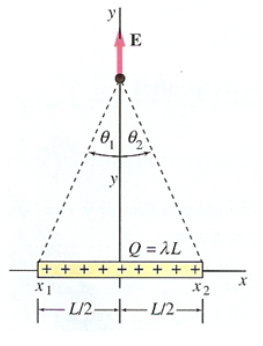
\includegraphics[width=0.17\textwidth]{Captura3.PNG}
    \end{wrapfigure} 

    \vspace{0.4cm}Para el caso de una distribución lineal de carga uniforme de longitud L en un punto P exterior situado en su mediatriz. En este caso el campo tiene una componente paralela a la carga lineal y otra perpendicular a ésta. Sin embargo, dada la simetría de la distribución cuando sumemos todos los elementos de carga de la línea, los componentes paralelos se anularán y el campo estará dirigido a lo largo del eje y. Por lo tanto, debido a la simetría, las componentes paralelas se anularán, haciendo que el campo este dirigido a lo largo del eje y.
    
    \vspace{0.6cm}El resultado es el siguiente:
    \vspace{-0.62cm}\begin{equation}
        \centering
        E_{y}=\frac{KQ}{y}\frac{1}{\sqrt{\left( \frac{L}{2}\right )^{2}+y^2}}
    \end{equation}
    
\subsection{Potencial eléctrico}
    El potencial eléctrico es una magnitud escalar que representa el trabajo a realizar por unidad de carga para mover dicha carga dentro de un campo eléctrico desde su punto inicial al punto considerado. 
    
    \vspace{5mm}
    También podemos interpretarla como la energía potencial eléctrica que adquiere una unidad de carga positiva al situarla en un punto de un campo eléctrico.

    \begin{equation}
        \centering
        E_{p}=K\cdot\frac{Q\cdot q}{r}
        \label{Ec:Ep}
    \end{equation}

    \begin{equation}
        \centering
        V=\frac{E_{p}}{q'}=\frac{K\frac{q\cdot q'}{r}}{q'}\  \Rightarrow \ V=K\cdot \frac{q}{r}
        \label{Ec:V}
    \end{equation}

\subsection{El dipolo eléctrico}
    El dipolo eléctrico elemental está formado por dos cargas iguales y de signo opuesto, separadas una distancia “d” mucho menor que las distancias macroscópicas que manejamos. Dicho de otro modo, se trata de conocer el valor del potencial o el campo de un par de cargas puntuales separadas una distancia $d$ en un punto $r$ tal que $r>>d$.
    \vspace{5mm}
    \newline Para la práctica calcularemos el potencial de un dipolo, por ello el potencial del par de cargas es:
    
    \begin{equation}
        \centering
        V = V_{+} + V_{-}=\frac{1}{4\pi\epsilon_{0}}\left ( \frac{+q}{r_{+}}+\frac{-q}{r_{-}}\right )
        \label{Ec:Vdipolo}
    \end{equation}

\subsection{Ecuación de Poisson}
    Es una ecuación en derivadas parciales con una amplia utilidad en electrostática. Un enfoque útil para el cálculo de los potenciales eléctricos que se refieren a la posibilidad de la densidad de la carga que da lugar a la misma.  El campo eléctrico está relacionado con la densidad de carga por la divergencia relación.

    \begin{equation}
        \Delta \cdot E = \frac{\rho}{\epsilon_{0}}
    \end{equation}

    El campo eléctrico está relacionado con el potencial eléctrico de un gradiente de relación:

    \begin{equation}
        E =- \nabla V
    \end{equation}    

\section{Resultados y discusión}
    Para la realización  del cálculo numérico necesario para hacer las simulaciones hemos empleado un programa en python, el cual viene adjuntado junto con este informe, en el se encuentra todo el código comentado y explicado. En este informe nos centraremos en los resultados obtenidos.

\subsection{Dipolo eléctrico}
        \begin{wrapfigure}[10]{l}{0.4\textwidth}
            \vspace{-0.6cm}
            \centering
            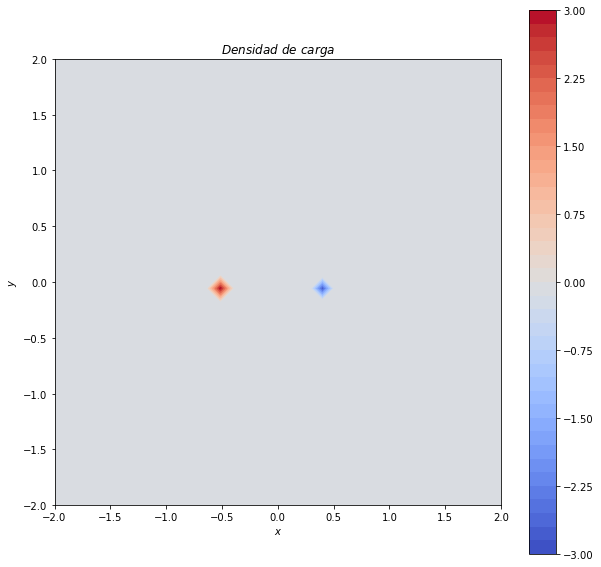
\includegraphics[width=0.36\textwidth]{dipolo1.PNG}
            \caption{Distribución de cargas}
            \label{fig:distr_cargas}
        \end{wrapfigure}
   
    \vspace{0.4cm}En la figura (\ref{fig:distr_cargas}) hemos representado un dipolo eléctrico,en ella podemos ver como están colocadas las cargas en el espacio, situando una carga negativa de -3C en la posición (-0.5,0,0) y una carga positiva de 3C en la posición (0.5,0,0).
        
    \vspace{0.4cm} En la figura (\ref{fig:potencial}) observamos el potencial eléctrico de nuestro dipolo desde el eje OX en la parte izquierda, y desde el eje OY en la parte derecha. Vemos como, acorde con su signo, las cargas provocan una cresta en el lugar de la positiva y un valle en el lugar de la negativa.

    \clearpage
    \begin{figure}[h]
        \centering
        \vspace{-1cm}
        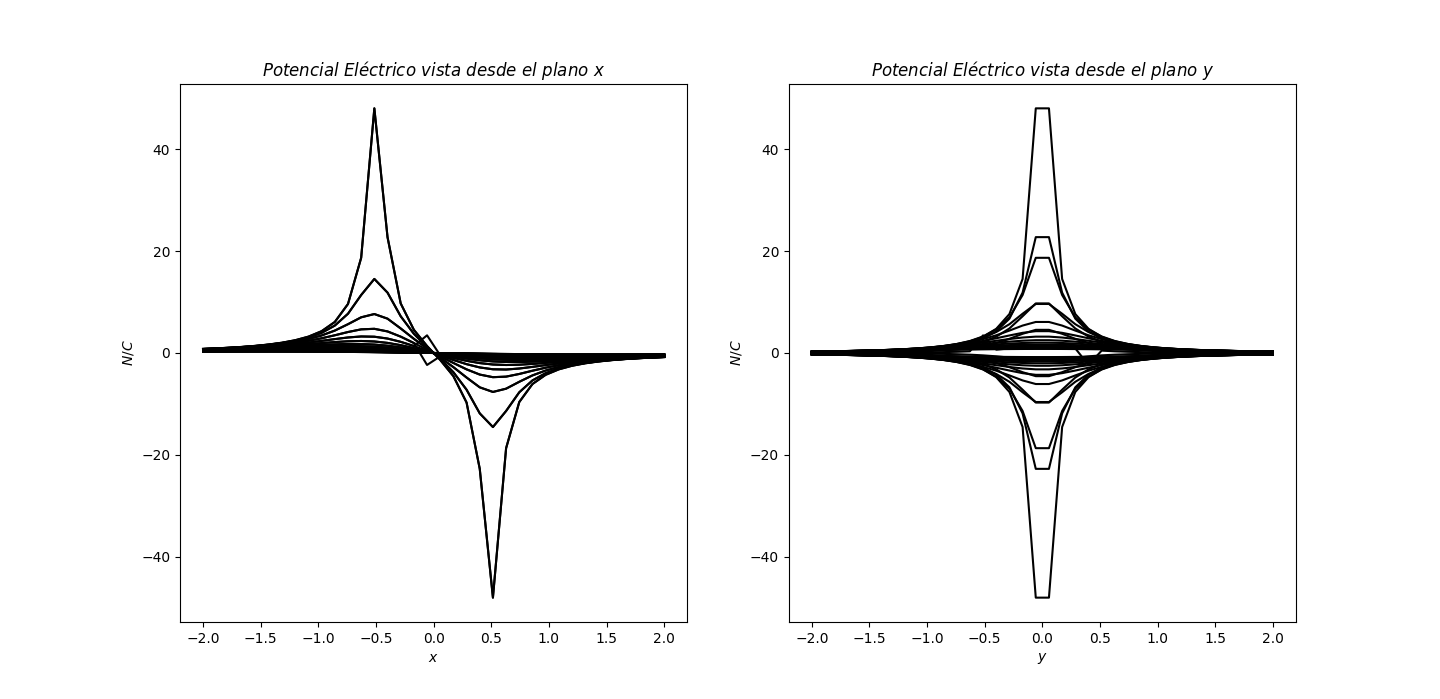
\includegraphics[width=0.65\textwidth]{dipolo2.png}
        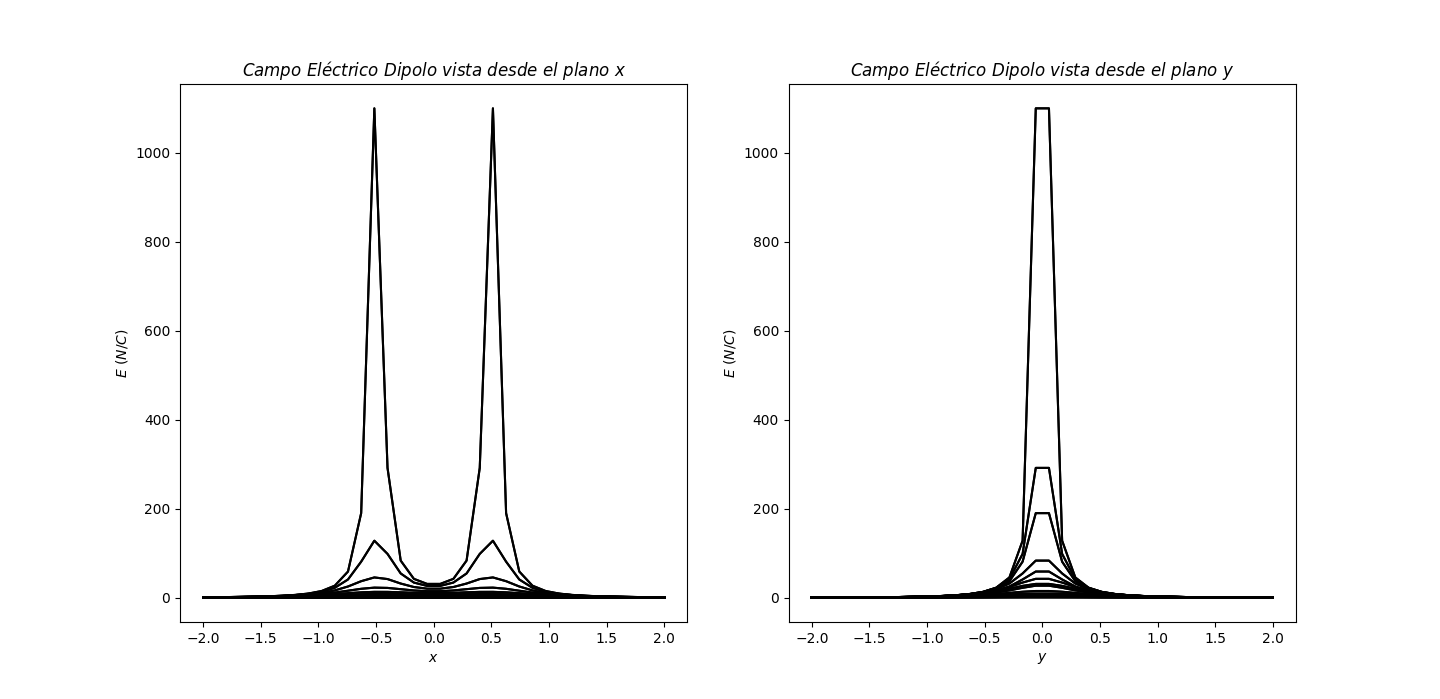
\includegraphics[width=0.65\textwidth]{dipolo3.PNG}
        \caption{Potencial eléctrico y Campo eléctrico (en valor absoluto)}
        \label{fig:potencial}
    \end{figure}

    Podemos comparar estos resultados a los que obtendríamos de forma analítica. Como observamos en la ecuación (\ref{Ec:Vdipolo}), cuando nos encontramos a la misma distancia de ambas cargas, el potencial es nulo. Esto mismos resultados son los que hemos obtenido de forma numérica, puesto que en el centro de la Figura 2, se aprecia como el potencial es igual a 0.
    
    \vspace{0.4cm} Es muy apreciable el decaimiento del campo eléctrico a medida que nos alejamos de las cargas, ya que como vimos en la ecuación (3), el campo disminuye con el cuadrado de la distancia.

    \begin{figure}[h]
        \vspace{-1cm}
        \centering
        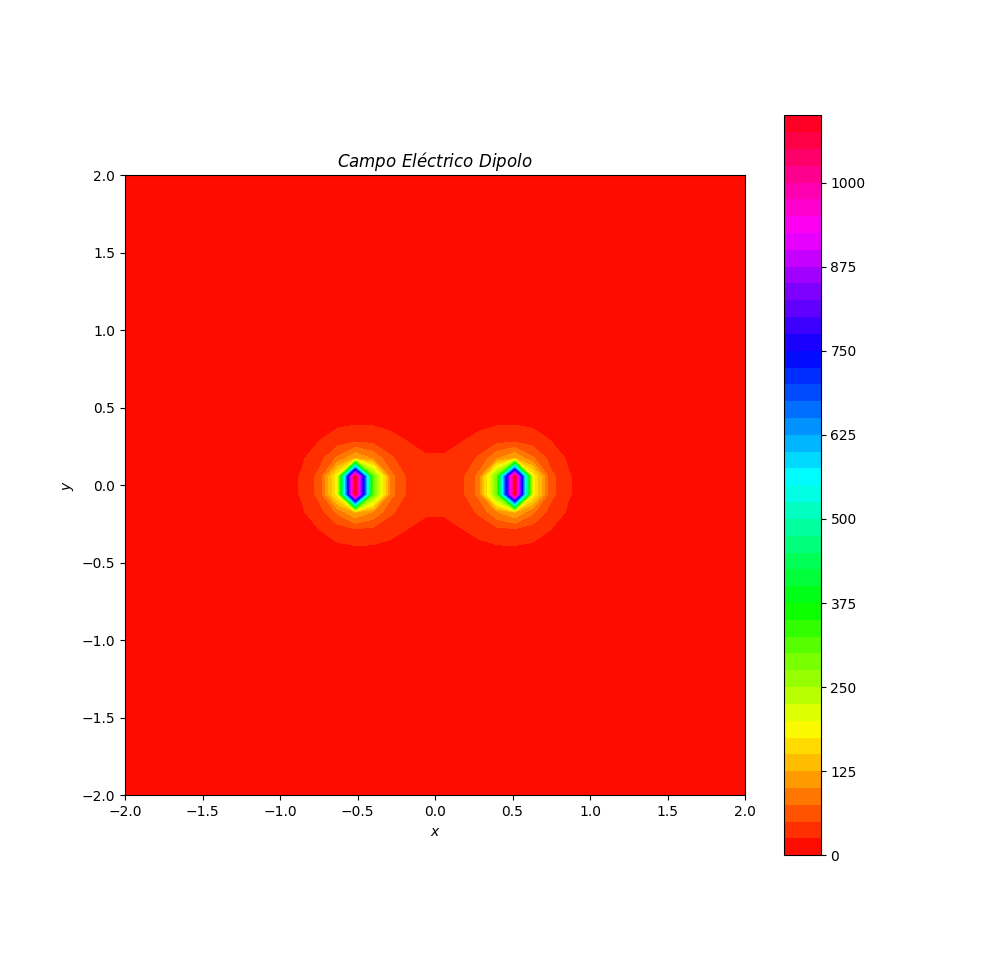
\includegraphics[width=0.44\textwidth]{dipolo4.PNG} 
        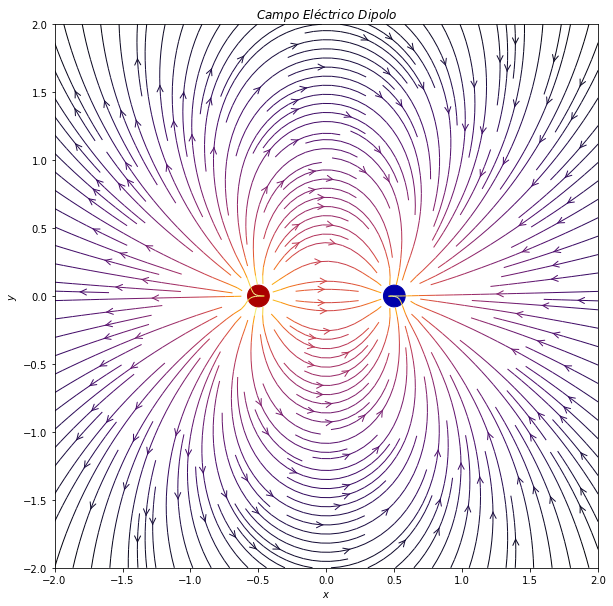
\includegraphics[width=0.35\textwidth]{dipolo 5.PNG}
    \end{figure}
    
    \vspace{0.4cm} A la izquierda tenemos la representación del campo eléctrico en forma escalar, es decir, nos muestra una escala de intensidades de valor del campo eléctrico. Y a la derecha tenemos una representación vectorial del campo eléctrico, es decir, se nos muestra la dirección que está tomando el campo, mediante la representación de sus líneas de campo. 

\clearpage
\subsection{Potencial y campo eléctrico debido a diferentes distribuciones de carga}
    En este apartado visualizaremos como se comporta el campo magnético y el potencial magnético en diferentes distribuciones de carga. Mediante algunas variaciones en nuestro código de python para el dipolo logramos distribuir las cargas en diferentes formas y orientaciones. A continuación mostramos algunas de ellas.

\vspace{-0.2cm}
\subsubsection{Distribución cuadrada}
    Para una distribución cuadrada de cargas obtenemos la siguiente representación:
    
    \vspace{0.2cm}\begin{figure}[h]
        \centering
        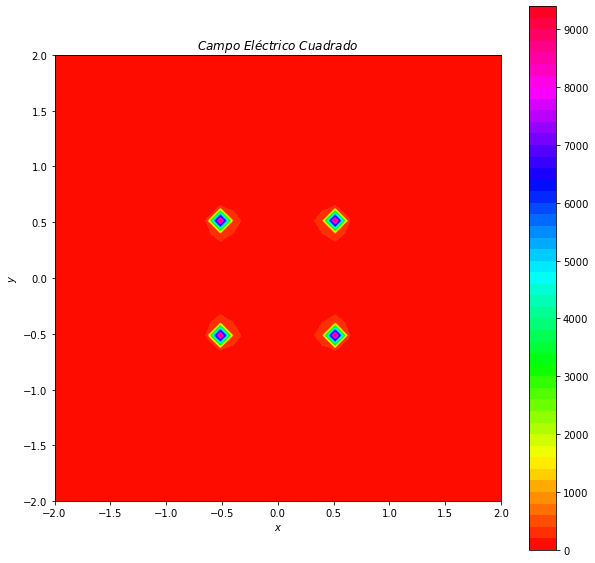
\includegraphics[width=0.45\textwidth]{cuadrado2.png}
        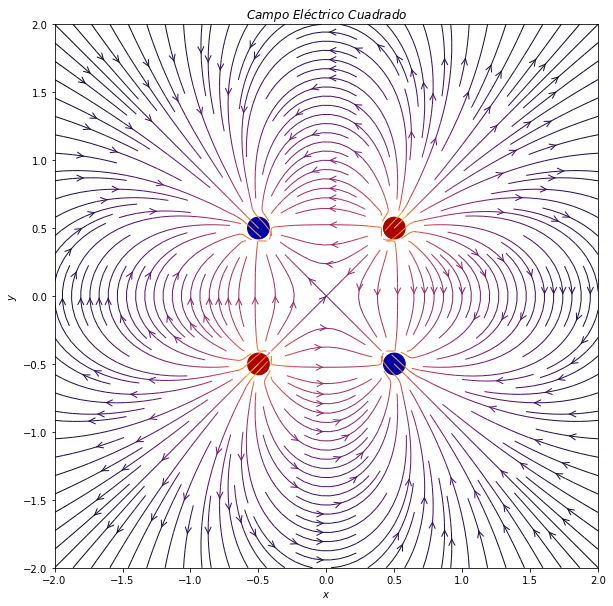
\includegraphics[width=0.42\textwidth]{cuadrado3.png}
    \end{figure}
    
    \vspace{0.4cm} A la izquierda vemos el campo escalar eléctrico y a la derecha el campo vectorial eléctrico generado por la distribución cuadrada de carga. Observamos como las lineas de campo se dirigen de las cargas positivas (puntos rojos) a las cargas negativas (puntos azules), tal y como debería ser. 

    \vspace{0.2cm}
        \begin{figure}[h]
            \centering
            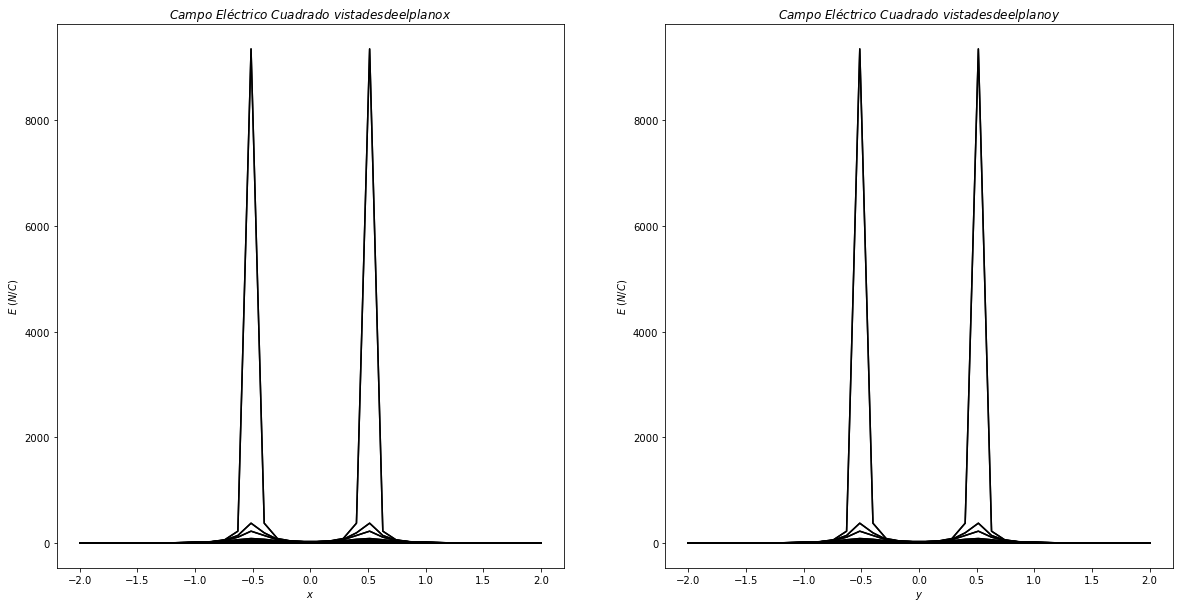
\includegraphics[width=0.7\textwidth]{cuadrado1.png}
            \caption{Campo eléctrico en valor absoluto distribución cuadrada}
        \end{figure}
        
    Debido a la simetría de la distribución de carga obtenemos la misma representación tanto para el eje OX como para el OY.

    \clearpage

\subsubsection{Distribución lineal}
    \vspace{5mm}Para una distribución lineal de cargas podemos distinguir dos casos, el caso donde la corriente filamental es finita y el caso donde es infinita. 

    \vspace{5mm}Para este caso será interesante la comparación de el hilo finito frente al hilo infinito.

    \vspace{0.8cm}\begin{tabular}{lr}
        \centering
        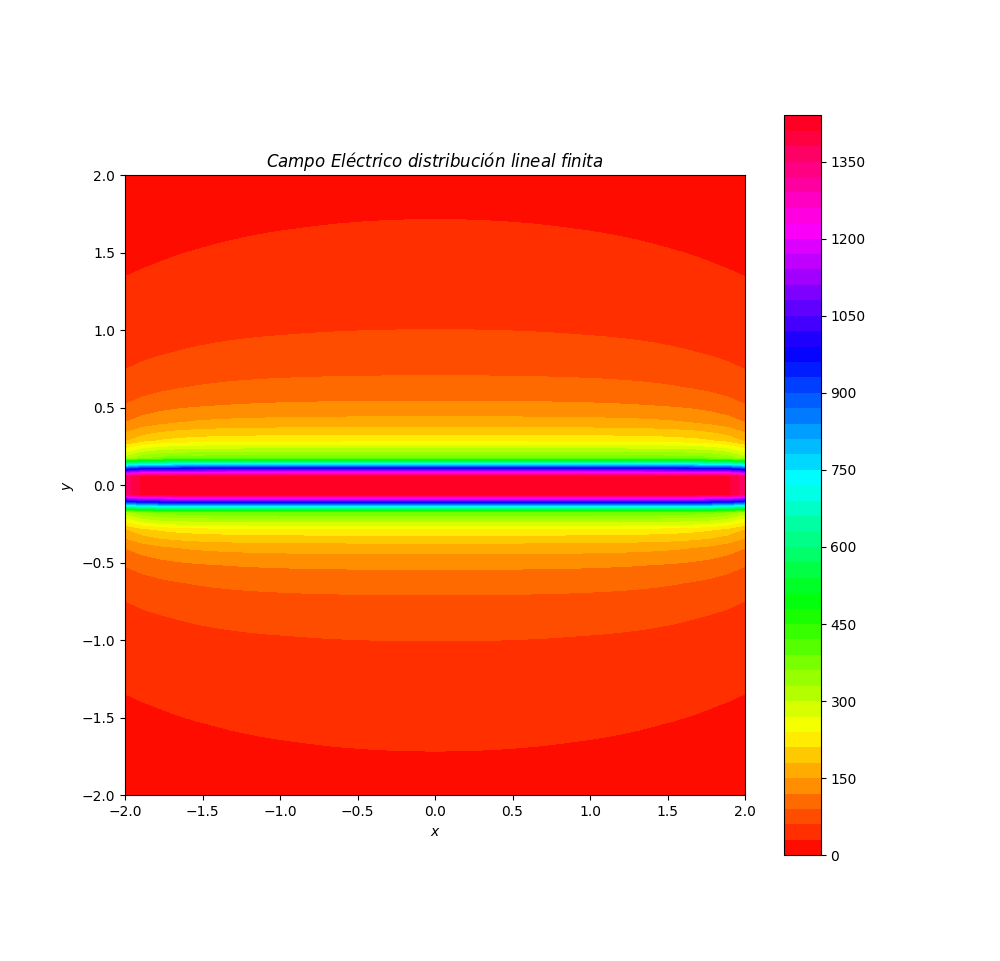
\includegraphics[width=0.45\textwidth]{finita2.png} &      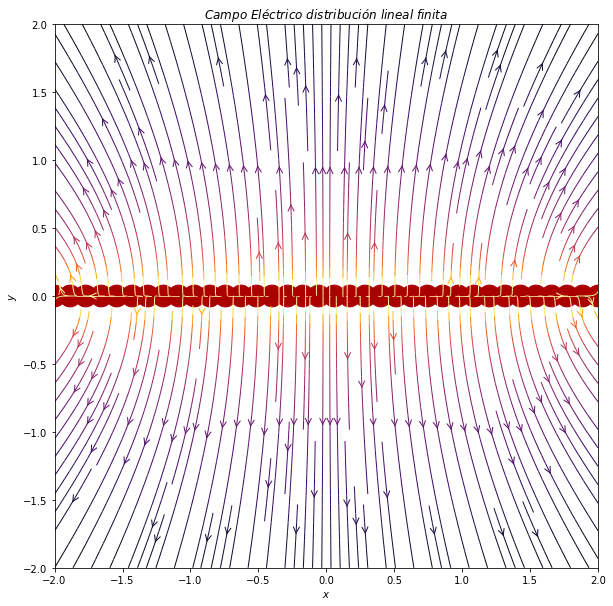
\includegraphics[width=0.45\textwidth]{finita3.png}
    \end{tabular}
    \vspace{1mm} 
    \begin{center}
     
         Hilo de corriente finita
    \end{center}
    
    \vspace{0.8cm}\begin{tabular}{lr}
        \centering
        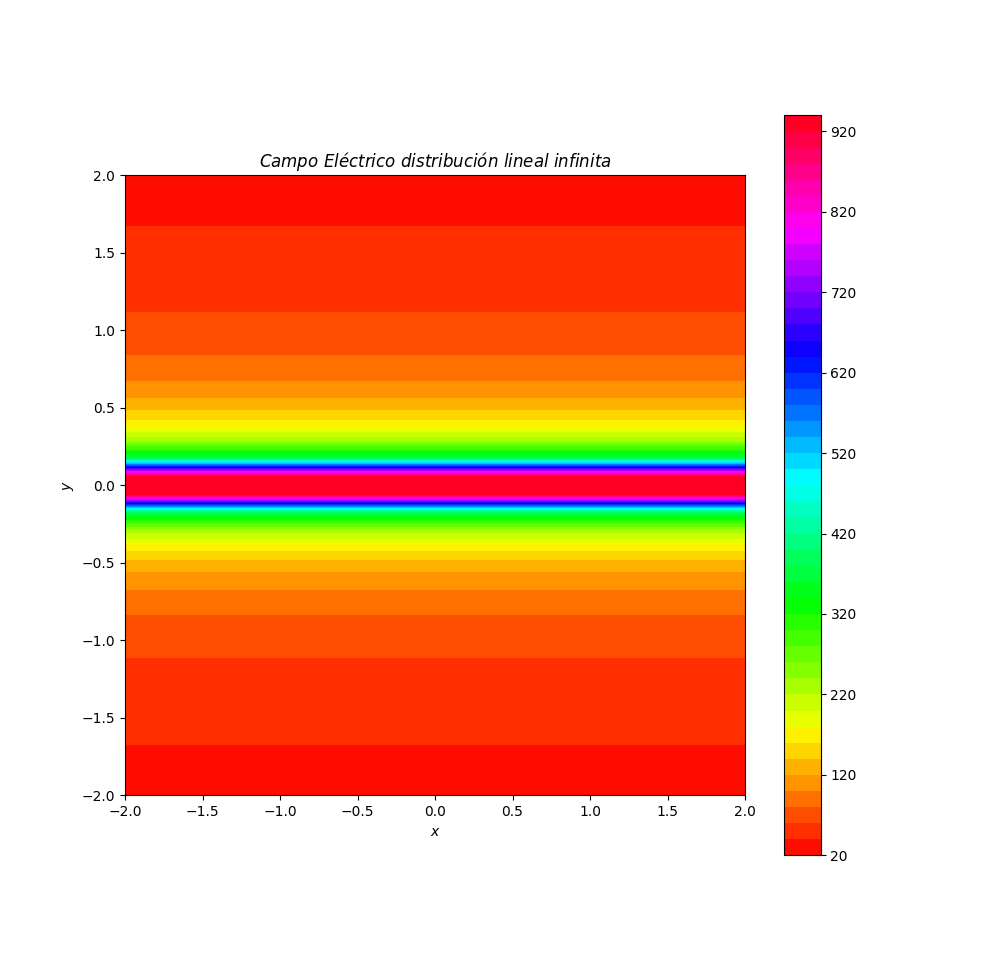
\includegraphics[width=0.45\textwidth]{infinita2.png} &      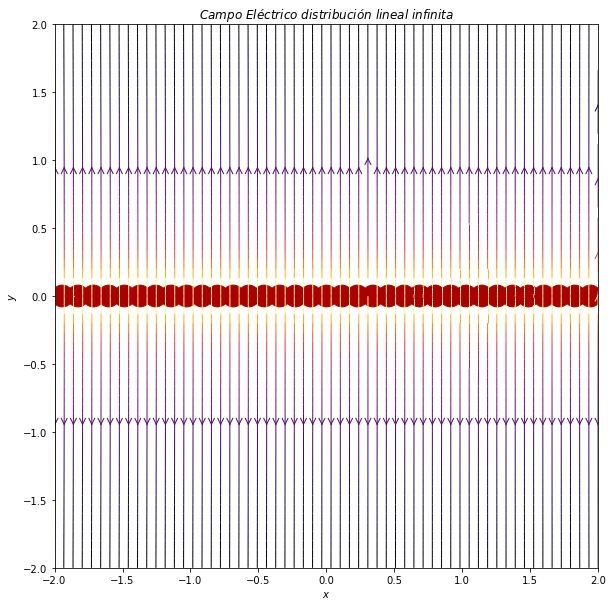
\includegraphics[width=0.45\textwidth]{infinita3.png}
    \end{tabular}
    \vspace{1mm} \begin{center}
         Hilo de corriente infinita
    \end{center}

    \clearpage
        \begin{figure}[h]
            \centering
            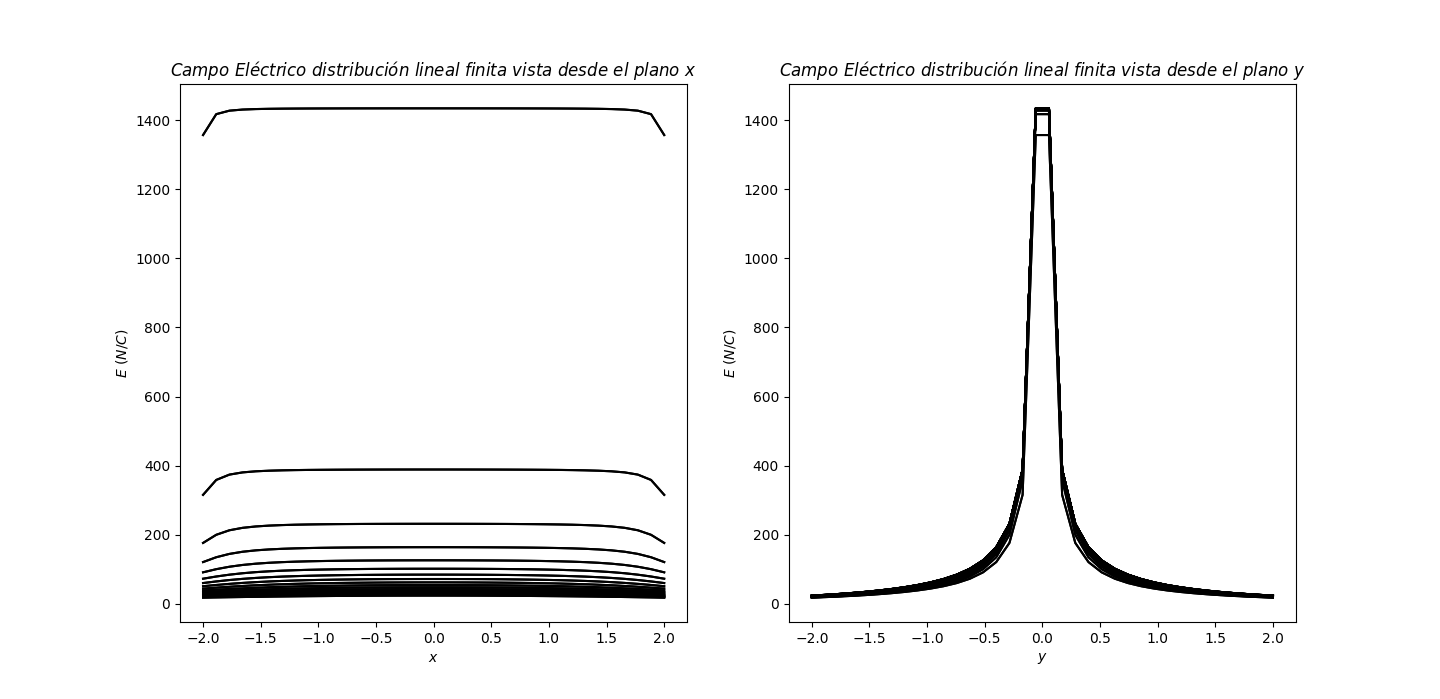
\includegraphics[width=0.6\textwidth]{finita1.png}
            \caption{Campo eléctrico hilo finito}
        \end{figure}

        \begin{figure}[h]
            \centering
            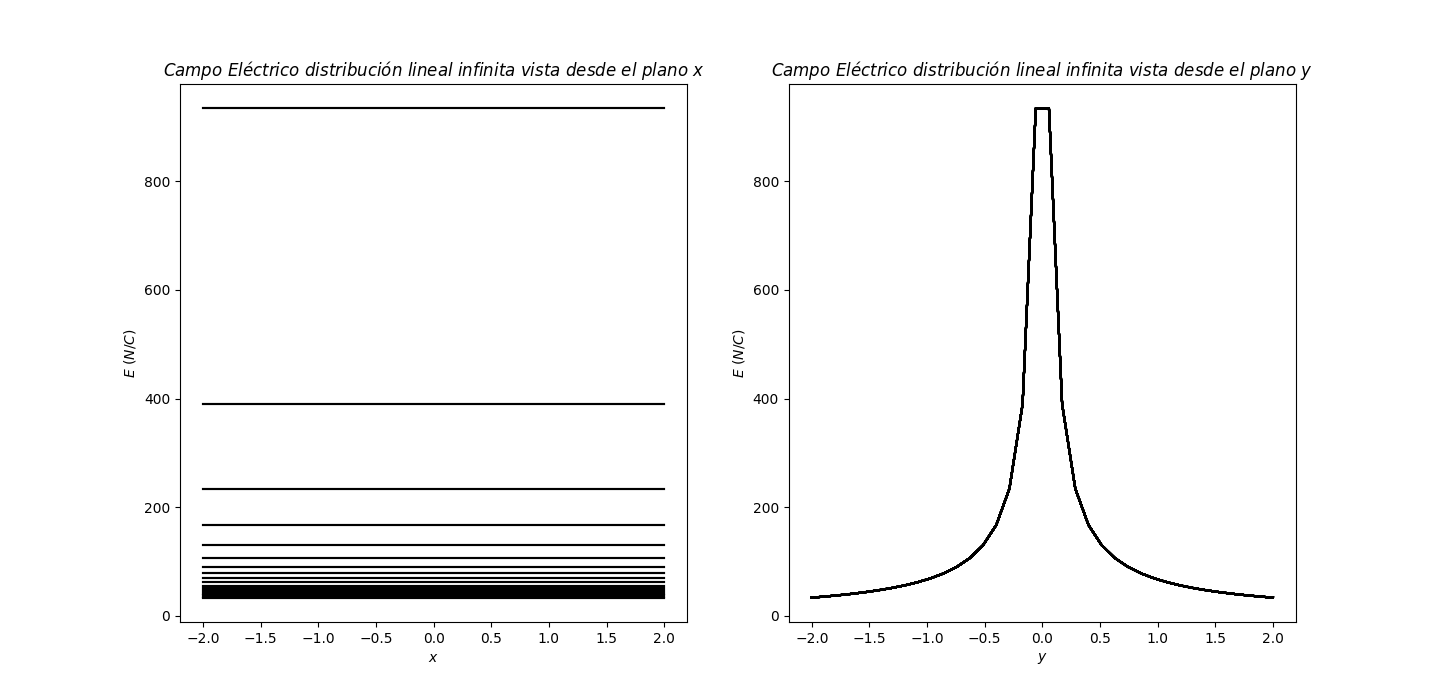
\includegraphics[width=0.6\textwidth]{infinita1.png}
            \caption{Campo eléctrico hilo infinito}
        \end{figure}

    \vspace{5mm} Estos dos casos son muy interesantes, puesto que aún siendo una distribución de cargas muy parecida, cuenta con diferencias muy notables. Fijándonos en los campos vectoriales, en la distribución finita, las lineas de campo se curvan, debido a que las componentes horizontales de las cargas de los extremos no logran cancelarse por completo. En cambio, en la distribución de carga infinita, si que se logra esa cancelación de las componentes horizontales del campo, creando un campo eléctrico completamente vertical. Para el campo escalar se puede apreciar el mismo efecto.


    \vspace{5mm} Este resultado también se resalta en las gráficas del campo eléctrico enfrentado a la distancia, haciendo que el campo eléctrico disminuya conforme a la distancia.

    \clearpage 

\subsubsection{Distribución circular}

    \begin{figure}[h]
        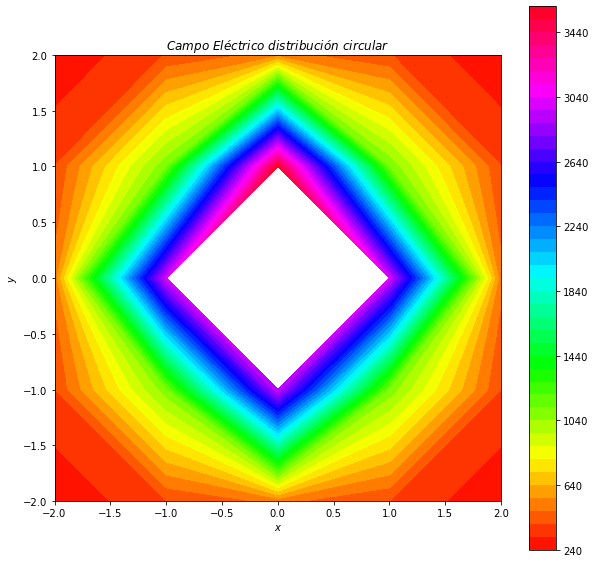
\includegraphics[width=0.25\textwidth]{circulo2.png}
        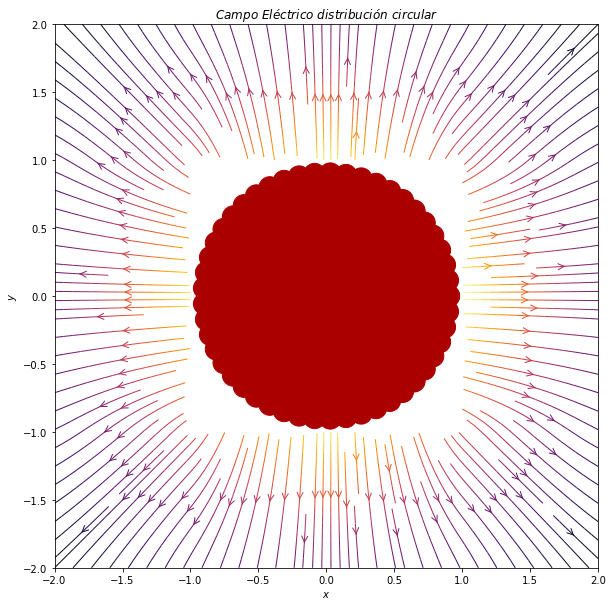
\includegraphics[width=0.25\textwidth]{circulo3.png}
        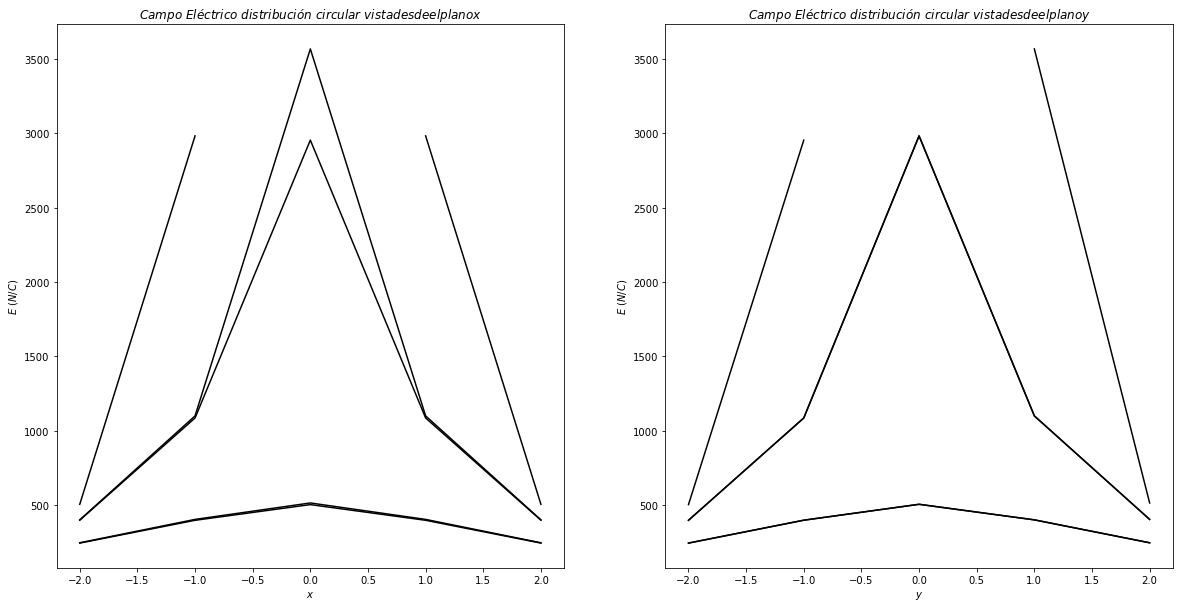
\includegraphics[width=0.5\textwidth]{circulo1.png}
        \caption{Distribución en círculo de las cargas}
    \end{figure}

    \begin{figure}[h]
        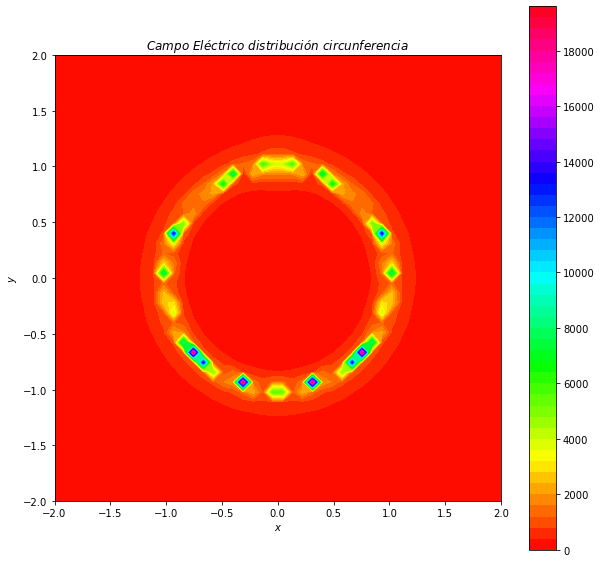
\includegraphics[width=0.25\textwidth]{circunferencia2.png}  
        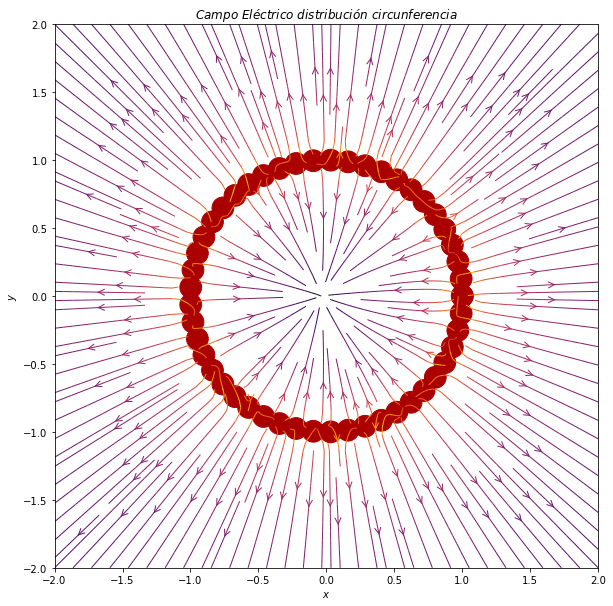
\includegraphics[width=0.25\textwidth]{circunferencia3.png}
        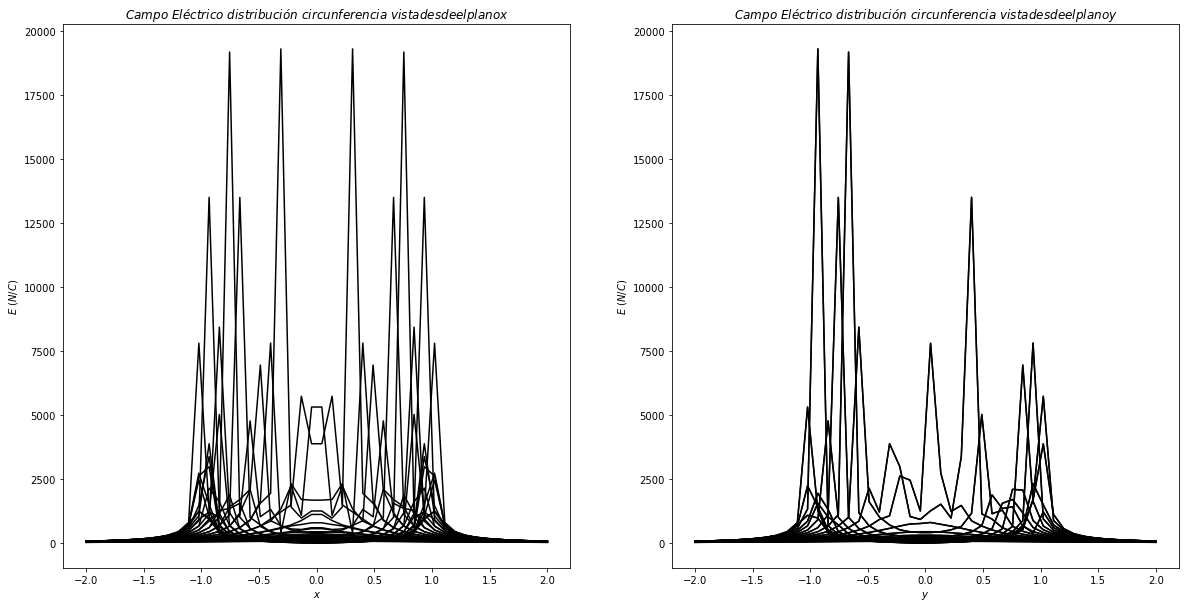
\includegraphics[width=0.5\textwidth]{circunferencia1.png}
        \caption{Distribución en circunferencia de las cargas}
    \end{figure}
        
    
    \vspace{5mm} La distribución circular es interesante, puesto que como podemos ver el campo eléctrico generado es radial y apunta hacia afuera del círculo. Comparando el círculo con la circunferencia, la principal diferencia es la intensidad del campo eléctrico. Lo podemos apreciar ampliamente en el gráfico que nos muestra el campo escalarmente, siendo este mucho más intenso en el caso del círculo. Esto se debe a que tenemos una mayor densidad de cargas en el círculo que en la circunferencia, por lo tanto hay más cargas que aportan al incremento del campo eléctrico.

\clearpage
\subsection{Resolución mediante la ecuación de Poisson}

\vspace{5mm} Para este apartado, resolveremos la ecuación de Poisson, la cual es muy útil para calcular el potencial eléctrico así como del campo eléctrico.

\vspace{5mm} Mediante una función programada en python y empleando el método de Jacobi, resolveremos la ecuación de Poisson para así lograr obtener el valor analítico del potencial eléctrico derivado de una distribución de cargas. Además, será necesario establecer que el potencial sea nulo en los bordes de su dominio.

\begin{figure}[h]
            \centering
            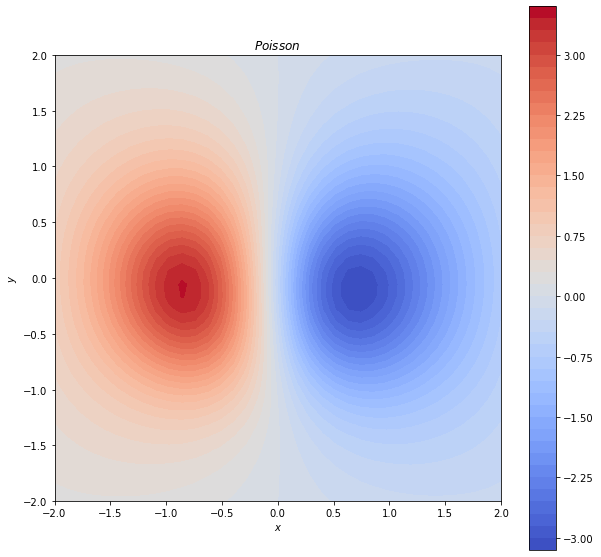
\includegraphics[width=0.4\textwidth]{poisson.png}
            \caption{Potencial debido a un dipolo}
        \end{figure}

\section{Anexos}
\subsubsection*{Código de python que genera las gráficas:}
\href{https://github.com/vmr48-ua/extras/blob/main/ELEC1-P1.py}{ELEC1-P1.py}
\subsubsection*{Código de LaTeX que genera este documento:}
\href{https://www.overleaf.com/read/bcpdkynrkkqs}{ELEC1-Práctica1:-Campos-Eléctricos.tex}
\end{document} 